\documentclass[10pt, a4paper,spanish]{article}

\usepackage[utf8]{inputenc}
\usepackage[spanish]{babel}

\usepackage[T1]{fontenc}

\usepackage[hmarginratio=1:1,top=32mm,columnsep=20pt]{geometry}
\usepackage[hang, small,labelfont=bf,up,textfont=it,up]{caption}


\usepackage{graphicx}
\graphicspath{ {images/} }

\usepackage{titlesec}
\renewcommand\thesection{\Roman{section}}
\renewcommand\thesubsection{\Roman{subsection}}
\titleformat{\section}[block]{\large\scshape\centering}{\thesection.}{1em}{}
\titleformat{\subsection}[block]{\large}{\thesubsection.}{1em}{}

\usepackage{fancyhdr}
\pagestyle{fancy}
\fancyhead{}
\fancyfoot{}
\fancyhead[C]{ \today \ $\bullet$ Minería de Datos $\bullet$ Lógica y Representación del Conocimiento}
\fancyfoot[RO]{\thepage}

%-------------------------------------------------------------------------------
%	TITLE SECTION
%-------------------------------------------------------------------------------

\title{\vspace{-15mm}\fontsize{24pt}{10pt}\selectfont\textbf{Lógica y Representación del Conocimiento}} % Article title

\author{Sergio García Prado}
\date{\today}

%-------------------------------------------------------------------------------

\begin{document}

	\maketitle % Insert title

	\thispagestyle{fancy} % All pages have headers and footers

%-------------------------------------------------------------------------------
%	TEXT
%-------------------------------------------------------------------------------

	\begin{center}
		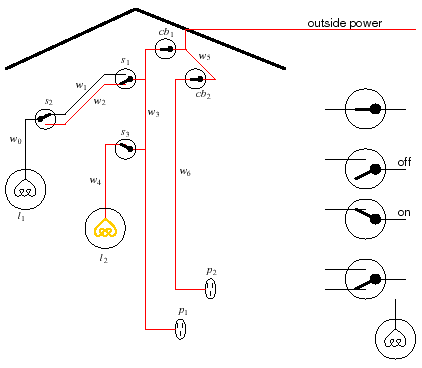
\includegraphics[width=0.6\textwidth]{diagnostic-assistant}
	\end{center}

	\section{Elaborar una base de conocimiento para el asistente al diagnóstico en el dominio del cableado de una vivienda. Las reglas generales deben de permitir codificar la instancia específica que muestra la figura. Utilizar los principios generales para la elaboración de una ontología específica.}


		\subsection{Vocabulario:}
			\begin{itemize}
				\item Constantes:
				\begin{itemize}
					\item $On$ y $Off$: Utilizadas para  representan si hay corriente en un componente.
					\item $Up$ y $Down$: Utilizadas para representar si un conmutador está en una posición u otra.
					\item $CircuitBreaker$, $Switch$, $Light$, $PowerOutlet$, $Wire$: Utilizadas para diferenciar los distintos tipos de componentes.
					\item $CB_i, i \in \{1,2\}$: Cada uno de los diferenciales de la figura.
					\item $S_i \in \{1,2,3\}$:  Cada uno de los conmutadores de la figura.
					\item $L_i \in \{1,2\}$: Cada una de las bombillas de la figura.
					\item $PO_i \in \{1,2\}$: Cada uno de los enchufes de la figura.
					\item $W_i \in \{0,1,2,3,4,5,6\}$: Cada uno de los cables de la figura.
					\item $OutsidePower$: Conexión de corriente externa de la figura.
				\end{itemize}
				\item Predicados:
				\begin{itemize}
					\item $Light(x) \equiv$ La variable $x$ luce.
					\item $Electrize(x) \equiv$ La variable $x$ produce electricidad (para enchufes).
					\item $Ok(x) \equiv$ La variable $x$ presenta un funcionamiento correcto.
					\item $Connected(x, y) \equiv$ La variable $x$ está conectada a la variable $y$.
				\end{itemize}
				\item Funciones:
				\begin{itemize}
					\item $in(x) = y \equiv$ La entrada de $x$ es $y$.
					\item $out(x,y) = z \equiv$ La salida $y$ de $x$ es  $z$.
					\item $signal(x) = y \equiv$ La señal de $x$ es  $y $.
					\item $state(x) = y \equiv$ El estado de $x$ es $y$.
					\item $type(x) = y \equiv$ El tipo de $x$ es $y$.
				\end{itemize}
			\end{itemize}

		\subsection{Ontología general:}

			\begin{itemize}

				%types
				\item Restricciones de Tipos de Componentes:
				\begin{itemize}
					\item $ CircuitBreaker \neq Switch\neq Ligth \neq PowerOutlet \neq Wire   $
					\item $ \forall x [((type(x) = CircuitBreaker) \lor (type(x) = Switch) \lor (type(x) = Ligth) \lor (type(x) = PowerOutlet) \lor (type(x) = Wire))] $
				\end{itemize}
				% Connections
				\item Restricciones de Conexiones:
				\begin{itemize}
					\item $ On \neq Off $
					\item $ \forall x [((signal(x) = On) \lor (signal(x) = Off))] $
					\item $ \forall x \forall y [(Connected(x, y) \supset Connected(y, x))] $
					\item $ \forall x \forall y [(Connected(x, y) \land Ok(x) \land Ok(y) \supset (signal(x) = signal(y)))] $
				\end{itemize}

				% Switchess
				\item Restricciones de Conmutadores:
				\begin{itemize}
					\item $ Up \neq Down $
					\item $ \forall x [( (state(x) = Up) \lor (state(x) = Down))] $
					\item $ \forall x [( ( (type(x) = Switch) \land (state(x) = Up) ) \supset Connected(in(x), out(x, Up)))] $
					\item $ \forall x [( ( (type(x) = Switch) \land (state(x) = Down) ) \supset Connected(in(x), out(x, Down)))] $
					\item $ \forall x [( (type(x) = Switch)  \supset Connected(in(x), out(x)))] $
				\end{itemize}

				% Circuit Breakers
				\item Restricciones de diferenciales:
				\begin{itemize}
					\item $ \forall x \forall y \forall z [( ((type(y) = CircuitBreaker) \land Connected(x, y) \land Connected(y, z) ) \supset Connected(x, z))] $
				\end{itemize}

				% Lights
				\item Restricciones de Bombillas:
				\begin{itemize}
					\item$ \forall x [(((signal(x) = On) \land (type(x) = Light) )  \supset Light(x))] $
				\end{itemize}

				% Power Outlets
				\item Restricciones de Enchufes:
				\begin{itemize}
					\item$ \forall x [(((signal(x) = On) \land (type(x) = PowerOutlet) )  \supset Electrize(x))] $
				\end{itemize}
			\end{itemize}

		\subsection{Ontología específica:}

			\begin{itemize}
				\item $ Ok(x),  x \in \{CB_i, S_j, L_k, PO_l, W_m, OutsidePower\}, i \in \{1,2\}, j \in \{1,2,3\},k \in \{1,2\},l \in \{1,2\},m \in \{1,2,3,4,5,6\}$
				\item $ type(CB_i) = CircuitBreaker, i \in \{1,2\} $
				\item $ type(S_i) = Switch, i \in \{1,2, 3\} $
				\item $ type(L_i) = Light, i \in \{1,2\} $
				\item $ type(PO_i) = PowerOutlet, i \in \{1,2\} $
				\item $ type(W_i) = Wire, i \in \{1,2, 3, 4, 5, 6\} $
				\item $ signal(OutsidePower) = On $
				\item $ state(S_1) = Down $
				\item $ state(S_2) = Up $
				\item $ state(S_3) = Up $
				\item $ Connected(OutsidePower, W_5)$
				\item $ Connected(W_5, CB_1)$
				\item $ Connected(W_5, CB_2)$
				\item $ Connected(CB_1, W_3)$
				\item $ Connected(CB_2, W_6)$
				\item $ Connected(W_6, PO_2)$
				\item $ Connected(W_3, PO_1)$
				\item $ Connected(W_3, in(S_1))$
				\item $ Connected(W_3, in(S_3))$
				\item $ Connected(out(S_3, Up), W_4)$
				\item $ Connected(W_4, L_2)$
				\item $ Connected(out(S_1, Up), W_1)$
				\item $ Connected(out(S_1, Down), W_2)$
				\item $ Connected(in(S_2), W_0)$
				\item $ Connected(W_0, L_1)$
			\end{itemize}



	\clearpage
	\section{Partiendo de la base de conocimiento del asistente al diagnóstico que hemos utilizado en las prácticas de la asignatura, elaborar la ontología que la soporta. Compararla con la ontología elaborada en el problema anterior.}

		\paragraph{}

		\subsection{Vocabulario:}
			\begin{itemize}
				\item Constantes:
				\begin{itemize}
					\item $CB_i, i \in \{1,2\}$: Cada uno de los diferenciales de la figura.
					\item $S_i \in \{1,2,3\}$:  Cada uno de los conmutadores de la figura.
					\item $L_i \in \{1,2\}$: Cada una de las bombillas de la figura.
					\item $P_i \in \{1,2\}$: Cada uno de los enchufes de la figura.
					\item $W_i \in \{0,1,2,3,4,5,6\}$: Cada uno de los cables de la figura.
					\item $Outside$: Conexión de corriente externa de la figura.
				\end{itemize}
				\item Predicados:
				\begin{itemize}
					\item $Light(x) \equiv$ La variable $x$ es una bombilla.
					\item $Lit(x) \equiv$ La variable $x$ luce.
					\item $Ok(x) \equiv$ La variable $x$ presenta un funcionamiento correcto.
					\item $Connected(x, y) \equiv$ La variable $x$ está conectada a la variable $y$.
					\item $ConnectedOk(x, y, z) \equiv$ La variable $x$ está conectada a la variable $y$ si la variable $z$ presenta un funcionamiento correcto.
					\item $ConnectedOkUp(x, y, z) \equiv$ La variable $x$ está conectada a la variable $y$ si la variable $z$ presenta un funcionamiento correcto y está en el estado $Up$.
					\item $ConnectedOkDown(x, y, z) \equiv$ La variable $x$ está conectada a la variable $y$ si la variable $z$ presenta un funcionamiento correcto y está en el estado $Down$.
					\item $Connected(x, y) \equiv$ La variable $x$ está conectada a la variable $y$.
					\item $Live(x) \equiv$ La variable $x$ tiene corriente.
					\item $Up(x) \equiv$ La variable $x$ en el estado up.
					\item $Down(x, y) \equiv$ La variable $x$ está en el estado down.
				\end{itemize}
			\end{itemize}

		\subsection{Ontología general:}

			\begin{itemize}
				\item $ \forall x [(Light(x) \land Ok(x) \land Live(x) \supset Lit(x)] $
				\item $ \forall x \forall y [(Connected(x, y) \land Live(x) \supset Live(y)] $
				\item $ \forall x \forall y \forall z [(ConnectedOk(x, y) \land Ok(z) \supset Connected(x, y)] $
				\item $ \forall x \forall y \forall z [(ConnectedOkUp(x, y) \land Ok(z) \land Up(z) \supset Connected(x, y)] $
				\item $ \forall x \forall y \forall z [(ConnectedOkDown(x, y) \land Ok(z) \land Down(z) \supset Connected(x, y)] $

			\end{itemize}

		\subsection{Ontología específica:}

			\begin{itemize}
				\item $ Ok(x),  x \in \{CB_i, S_j, L_k\}, i \in \{1,2\}, j \in \{1,2,3\},k \in \{1,2\}$
				\item $ Live(Outside)$
				\item $ Light(L_1)$
				\item $ Light(L_2)$
				\item $ Down(S_1)$
				\item $ Up(S_2)$
				\item $ Up(S_3)$
				\item $ Connected(L_1, W_0)$
				\item $ Connected(L_2, W_4)$
				\item $ Connected(P_1, W_3)$
				\item $ Connected(P_2, W_6)$
				\item $ Connected(W_5, Outside)$


				\item $ ConnectedOk(W_2, W_5, CB_1)$
				\item $ ConnectedOk(W_6, W_5, CB_2)$

				\item $ ConnectedOkUp(W_1, W_3, S_1$
				\item $ ConnectedOkDown(W_2, W_3, S_1)$

				\item $ ConnectedOkUp(W_0, W_1, S_2$
				\item $ ConnectedOkDown(W_0, W_2, S_2)$


				\item $ ConnectedOkUp(W_4, W_3, S_3)$
			\end{itemize}

\end{document}
